\documentclass[10pt]{standalone}
\usepackage[utf8]{inputenc}
\usepackage{pgf,tikz,pgfplots}
\pgfplotsset{compat=1.15}
\usepackage{mathrsfs}
\usetikzlibrary{arrows}
\pagestyle{empty}
\begin{document}

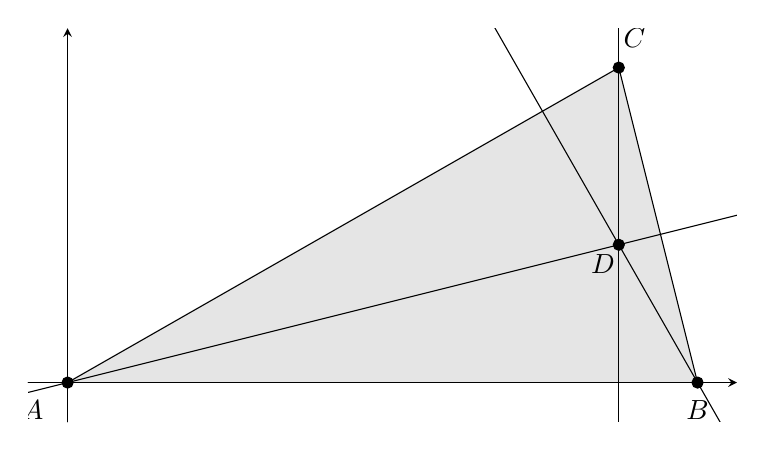
\begin{tikzpicture}[line cap=round,line join=round,>=triangle 45,x=1.0cm,y=1.0cm]
\begin{axis}[
x=1.0cm,y=1.0cm,
axis lines=middle,
ticks=none,
xmin=-0.5,
xmax=8.5,
ymin=-0.5,
ymax=4.5,]
\clip(-0.5,-0.5) rectangle (8.5,4.5);
\fill[color=black,fill=black,fill opacity=0.10000000149011612] (0.,0.) -- (7.,4.) -- (8.,0.) -- cycle;
\draw  (0.,0.)-- (7.,4.);
\draw  (7.,4.)-- (8.,0.);
\draw  (8.,0.)-- (0.,0.);
\draw  (7.,-0.5) -- (7.,4.5);
\draw [domain=-0.5:8.5] plot(\x,{(-0.--0.25*\x)/1.});
\draw [domain=-0.5:8.5] plot(\x,{(--14.-1.75*\x)/1.});
\begin{scriptsize}
\draw [fill=black] (0.,0.) circle (2.0pt);
\draw (-0.44,-0.35) node {$A$};
\draw [fill=black] (7.,4.) circle (2.0pt);
\draw (7.2,4.37) node {$C$};
\draw [fill=black] (8.,0.) circle (2.0pt);
\draw (8.0,-0.35) node {$B$};

\draw [fill=black] (7.,1.75) circle (2.0pt);
\draw[color=black] (6.8,1.5) node {$D$};
\end{scriptsize}
\end{axis}
\end{tikzpicture}
\end{document}